\documentclass[border=4pt,12pt]{standalone}
% House style for redrawn exam diagrams (diagram-v4: 0.4pt lines, filled -latex arrows, fine dashes; stipple and hatching drawn as real dots/lines (no PDF/SVG patterns, so they render in every browser and at any scale); transparent background). Every figure \input's this.
\usepackage{amsmath,amssymb}
\usepackage{txfonts}
\usepackage{pdfrender,xcolor}
% \halo{text}: label on shading. The shading stops just around each letter's outline (a thin knock-out that follows the
% glyphs, like the papers' typesetting), never a box. Owner: "I don't want a box around the text".
\newcommand{\halo}[1]{\leavevmode\rlap{\pdfrender{TextRenderingMode=2,LineWidth=2.2pt,LineJoinStyle=1,StrokeColor=white,FillColor=white}#1}#1}
\usepackage{tikz,pgfplots}
\pgfplotsset{compat=1.18}
\usetikzlibrary{arrows.meta,calc,angles,quotes,patterns,patterns.meta,intersections,positioning,decorations.markings,shapes.geometric}
% Stipple and hatching are drawn as actual dots / lines clipped to the region (path picture), NOT as pattern fills:
% SVG <pattern> fills vanish or blur when browsers scale the image, so the owner could not see the shading.
% Each dot is a 0.72pt square (keeps SVGs small; reads as a dot at print size). Dots sit on one global staggered grid, so neighbouring regions line up.
\makeatletter
\newdimen\ex@x \newdimen\ex@y \newdimen\ex@xa \newdimen\ex@ya \newdimen\ex@xb \newdimen\ex@yb \newcount\ex@row
\def\exam@stipplecolor{black!75}\def\exam@dotr{0.42pt}\def\exam@dotgap{2.5}
\def\ex@rowdots{\ifdim\ex@x<\ex@xb \pgfpathrectangle{\pgfqpoint{\dimexpr\ex@x-0.36pt\relax}{\dimexpr\ex@y-0.36pt\relax}}{\pgfqpoint{0.72pt}{0.72pt}}\advance\ex@x by \exam@dotgap pt\relax\expandafter\ex@rowdots\fi}
\def\exam@stipple{%
  \pgftransformreset% dots are sized in real points even inside scaled pictures
  \pgfpointanchor{path picture bounding box}{south west}\ex@xa=\pgf@x \ex@ya=\pgf@y
  \pgfpointanchor{path picture bounding box}{north east}\ex@xb=\pgf@x \ex@yb=\pgf@y
  \pgfsetfillcolor{\exam@stipplecolor}\pgfmathsetmacro\ex@h{\exam@dotgap/2}%
  \pgfmathtruncatemacro\ex@r{floor(\ex@ya/\ex@h)-1}\ex@row=\ex@r\relax
  \ex@y=\ex@r\dimexpr\ex@h pt\relax
  \loop\ifdim\ex@y<\ex@yb
    \pgfmathtruncatemacro\ex@c{floor(\ex@xa/\exam@dotgap)-1}\ex@x=\ex@c\dimexpr\exam@dotgap pt\relax
    \ifodd\ex@row \advance\ex@x by \ex@h pt\fi
    \ex@rowdots
    \advance\ex@y by \ex@h pt \advance\ex@row by 1
    \ifnum\numexpr\ex@row-(\ex@row/4)*4\relax=0 \pgfusepath{fill}\fi% flush every 4 rows: bounded TeX memory, few clip copies in the SVG
  \repeat\pgfusepath{fill}}
\newdimen\ex@d
\def\exam@hatch#1{% #1 = 1 for /, -1 for \ ; lines 45 degrees, 3pt apart
  \pgftransformreset
  \pgfpointanchor{path picture bounding box}{south west}\ex@xa=\pgf@x \ex@ya=\pgf@y
  \pgfpointanchor{path picture bounding box}{north east}\ex@xb=\pgf@x \ex@yb=\pgf@y
  \ex@d=\dimexpr\ex@yb-\ex@ya\relax \ex@x=\dimexpr\ex@xa-\ex@d\relax
  \loop\ifdim\ex@x<\ex@xb
    \ifnum#1>0 \pgfpathmoveto{\pgfqpoint{\ex@x}{\ex@ya}}\pgfpathlineto{\pgfqpoint{\dimexpr\ex@x+\ex@d\relax}{\ex@yb}}%
    \else \pgfpathmoveto{\pgfqpoint{\ex@x}{\ex@yb}}\pgfpathlineto{\pgfqpoint{\dimexpr\ex@x+\ex@d\relax}{\ex@ya}}\fi
    \advance\ex@x by 4.24pt
  \repeat
  \pgfsetlinewidth{0.4pt}\pgfsetstrokecolor{black}\pgfusepath{stroke}}
\def\examstipple{\exam@stipple}\def\examhatch{\exam@hatch}\def\examsetstipplecolor#1{\def\exam@stipplecolor{#1}}\def\examsetdotgap#1{\def\exam@dotgap{#1}}
\makeatother
% (legacy pattern kept for old files)
% staggered stipple like the NESA papers' dotted shading
\pgfdeclarepatternformonly{exam stipple}{\pgfpointorigin}{\pgfqpoint{2.2pt}{2.2pt}}{\pgfqpoint{2.2pt}{2.2pt}}{%
  \pgfpathcircle{\pgfqpoint{0.55pt}{0.55pt}}{0.42pt}\pgfpathcircle{\pgfqpoint{1.65pt}{1.65pt}}{0.42pt}\pgfusepath{fill}}
\tikzset{
  every picture/.style={line width=0.6pt, >={Latex[length=2mm,width=1.3mm]}},
  curve/.style={line width=0.6pt},
  open arrow/.style={-{Latex[length=2mm,width=1.3mm]}},  % owner: filled -latex heads everywhere, no open chevrons
  aux/.style={dash pattern=on 2pt off 1.5pt, line width=0.6pt},
  shade/.code={\def\exA{#1}\def\exB{none}\ifx\exA\exB\else\pgfkeysalso{fill=black!18}\fi},
  shade/.default=on,
  shade dots/.style={fill=none, path picture={\examstipple}},
  stipple color/.code={\examsetstipplecolor{#1}},
  stipple gap/.code={\examsetdotgap{#1}},
  shade dense dots/.style={fill=none, stipple gap=1.6, path picture={\examstipple}},
  shade hatch/.style={fill=none, path picture={\examhatch{1}}},
  shade hatch reverse/.style={fill=none, path picture={\examhatch{-1}}},
  shade solid/.style={fill=black},
  pt/.style={circle, fill, inner sep=1.1pt},
  open pt/.style={circle, draw, fill=white, inner sep=1.1pt},
}
\pgfplotsset{
  exam axes/.style={axis lines=middle, axis line style={->}, xlabel={$x$}, ylabel={$y$},
    xlabel style={anchor=west}, ylabel style={anchor=south}, tick label style={font=\small},
    every axis plot/.append style={line width=0.6pt, black}, samples=200, clip=false,
    enlargelimits=false, axis on top},
}

\begin{document}
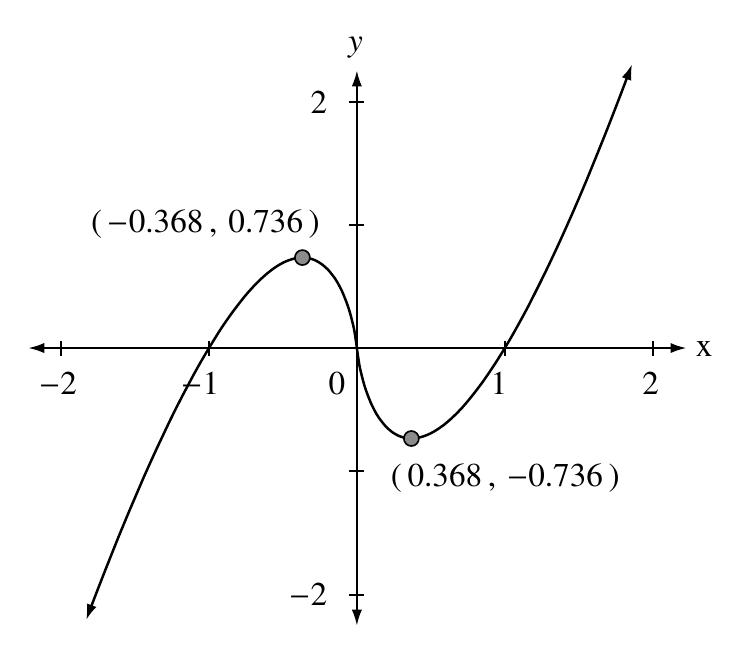
\begin{tikzpicture}[x=0.0127cm,y=-0.0127cm,font=\large]
  \draw[<->] (18,330.5) -- (676,330.5);
  \draw[<->] (346.5,608) -- (346.5,53);
  \foreach \i in {50.5,198.5,494.5,642.5}{\draw (\i,323) -- (\i,338);}
  \foreach \j in {84.5,207.5,453.5,577.5}{\draw (339,\j) -- (354,\j);}
  \node[anchor=base] at (47.5,377) {$-2$};
  \node[anchor=base] at (190,377) {$-1$};
  \node[anchor=base] at (326.5,377) {$0$};
  \node[anchor=base] at (488.5,377) {$1$};
  \node[anchor=base] at (640.5,377) {$2$};
  \node[anchor=east] at (327,84.5) {$2$};
  \node[anchor=east] at (327,577) {$-2$};
  \node at (345,30) {$y$};
  \node at (694,331) {x};
  \draw[<->,line width=0.9pt] plot[smooth] coordinates {(75.7,602.6) (82.0,585.7) (88.4,569.1) (94.8,552.7) (101.2,536.6) (107.5,520.8) (113.9,505.3) (120.3,490.0) (126.7,475.1) (133.0,460.4) (139.4,446.1) (145.8,432.1) (152.2,418.5) (158.5,405.2) (164.9,392.2) (171.3,379.6) (177.7,367.5) (184.0,355.7) (190.4,344.3) (196.8,333.4) (203.2,322.9) (209.5,312.8) (215.9,303.3) (222.3,294.3) (228.7,285.9) (235.0,278.0) (241.4,270.7) (247.8,264.0) (254.2,258.1) (260.5,252.9) (266.9,248.4) (273.3,244.8) (279.7,242.2) (286.0,240.5) (292.4,240.0) (298.8,240.7) (305.2,242.9) (311.5,246.7) (317.9,252.4) (324.3,260.5) (326.8,264.4) (329.2,268.8) (331.7,273.8) (334.1,279.5) (336.6,286.0) (339.1,293.5) (341.5,302.4) (344.0,313.4) (346.4,329.6) (346.5,330.5) (346.6,331.4) (349.0,347.6) (351.5,358.6) (353.9,367.5) (356.4,375.0) (358.9,381.5) (361.3,387.2) (363.8,392.2) (366.2,396.6) (368.7,400.5) (375.2,408.7) (381.7,414.5) (388.2,418.3) (394.7,420.4) (401.1,421.0) (407.6,420.3) (414.1,418.5) (420.6,415.7) (427.1,411.9) (433.6,407.3) (440.1,401.8) (446.6,395.6) (453.1,388.7) (459.5,381.1) (466.0,372.9) (472.5,364.2) (479.0,354.8) (485.5,345.0) (492.0,334.6) (498.5,323.8) (505.0,312.5) (511.5,300.7) (518.0,288.6) (524.4,276.0) (530.9,263.0) (537.4,249.7) (543.9,236.0) (550.4,221.9) (556.9,207.5) (563.4,192.8) (569.9,177.7) (576.4,162.3) (582.8,146.6) (589.3,130.6) (595.8,114.4) (602.3,97.8) (608.8,81.0) (615.3,63.9) (621.8,46.5)};
  \filldraw[fill=black!45] (292.0,240.0) circle (7.5) (401.0,421.0) circle (7.5);
  \node at (195,207) {$(\,-0.368\,,\,0.736\,)$};
  \node at (495,461) {$(\,0.368\,,\,-0.736\,)$};
\end{tikzpicture}
\end{document}
